\documentclass{llncs}
\usepackage{times}
\usepackage[T1]{fontenc}

% Comentar para not MAC Users
\usepackage[applemac]{inputenc}

\usepackage{a4}
%\usepackage[margin=3cm,nohead]{geometry}
\usepackage{epstopdf}
\usepackage{graphicx}
\usepackage{fancyvrb}
\usepackage{amsmath}
%\renewcommand{\baselinestretch}{1.5}

% CAPITAL LETTER LETTRINE
\usepackage{lettrine}

\begin{document}
\mainmatter
\title{Overview of Content-Delivery Networks Architecture}

\titlerunning{Paper Title}

\author{Afonso Silva\and Alfredo Gomes \and Axel Ferreira}

\authorrunning{Autor1 \and Autor2 \and Autor3}

\institute{University of Minho, Department of Informatics, 4710-057 Braga, Portugal\\
e-mail: \{a70387,a71655,a53064\}@alunos.uminho.pt
}

\date{\today}

\bibliographystyle{splncs}
%---------------- TITLE
\maketitle


%---------------- TABLE OF CONTENTS
%\tableofcontents
%\newpage



%%%%%%%%%%%%%%%%%%%%%%%%%%%%%%%%%%%%%%%%%%%%%%%%%%%%%%%%
%---------------- ABSTRACT							%(Axel)
%%%%%%%%%%%%%%%%%%%%%%%%%%%%%%%%%%%%%%%%%%%%%%%%%%%%%%%%
\begin{abstract}
	Given the diversity of existing Content Delivery Networks (CDN) architectures and the lack of a reference explicitly organising this information, this paper intends to overview three main CDN architectures. A description of Traditional Commercial \textit{CDN}s, Peer-to-Peer (P2P) \textit{CDN}s and Hybrid \textit{CDN}s is presented. For each architecture, the advantages, disadvantages, technical challenges and application scopes are presented.
	Implications for further research and practice are discussed.
\end{abstract}
%----------------





% \begin{multicols}{2}




%%%%%%%%%%%%%%%%%%%%%%%%%%%%%%%%%%%%%%%%%%%%%%%%%%%%%%%%
\section{Introduction}									%(Axel)
%%%%%%%%%%%%%%%%%%%%%%%%%%%%%%%%%%%%%%%%%%%%%%%%%%%%%%%%
%According to Table~\ref{tab:TabelaExemplo} \dots

	%\subsection{Context}
	\lettrine[lines=2]{T}{he} Internet has its origins in the early 1980's and presented an exponential growth when commercial companies started to link to the existing academic and military networks during the 90's. As the popularity of the Internet increased the number of devices connected started to see an exponential growth.\\ 
	% \subsection{Problems }
	At that time networks were unreliable and Internet communication protocols were designed in a robust fashion. As an example, Hypertext Transfer Protocol (HTTP) was designed to survive multiple packet losses and thus being a very chatty protocol, there are multiple Round-trip Time (RTTs) this causes a latency problem over long distance communication.
	Modern networks are faster and more reliable, but most of the core protocols mentioned above don't take advantage of the increased reliability. %(Due to Backwards compatibility)
	As the Internet role in daily life grew, new technologies star to emerge providing images videos and other dynamic content. This caused a bottleneck in servers with popular content.
	The above problems, led to the development Content Delivery Networks.

	%\subsection{What is a \textit{CDN}?}
	A \textit{CDN} is a large network of distributed storage servers which cash the content in multiple locations strategically spread. Traditionally \textit{CDN} servers are stored in ISP's facilities. This reduces both infrastructural costs to \textit{CDN} Providers and ISP's costs by keeping popular content local, in contrast to bringing it from another ISP's network.

	%\subsection{How does it Work?}
	A \textit{CDN} works by keeping a copy of the content in different locations. Whenever content is requested, management software calculates the best Server for accessing the content. This reduces distance to server which improves latency and minimizes packet loss. 
	Since the calculations are dynamic, in case of a server malfunction another Server is chosen, providing redundancy.
	
	%\subsection{ \textit{CDN} Service vs in House Solution}
	Traditional \textit{CDN} business model target bandwidth as a cost factor. This brings two advantages over a 'In House' solution:
	First, there are no initial infrastructural costs, this is a big advantage. An example of the dimension of such structure's size would be Akamai's infrastructure. It is composed by more than 61,000 servers, spread across 1000 networks in 70 countries worldwide\cite{akamai};
	Second, provides bandwidth on demand. In comparison with an 'In House' solution, there is no need to deal with both predictable and unpredictable traffic peaks.
	Due to its large distributed infrastructure, and high bandwidth on demand \textit{CDN}s are especially well suited to absorve a Denial of Service (DoS) attacks\cite{cdnetworks}.

	%\subsection{Costs}
	It is worth noting that \textit{CDN}s bring cost per performance down. Despite that, \textit{CDN}s are expensive, and currently are used mostly by big companies. It is imperative that \textit{CDN}'s get cheaper. This will allow more parties to use them, thus enhancing Internet experience to the final consumer and reducing total Internet traffic at the same time.
	% Exemplo (�mbito de aplica��o) Netflix
	An example of a service using a \textit{CDN} (Amazon EC2) would be the popular movie streaming service Netflix.


	\subsection{Purpose} %Prop�sito do paper
		
		This paper's purpose is to provide organised information about different \textit{CDN} architectures: the traditional large server infrastructure \textit{CDN}, the P2P \textit{CDN} and a new trend of Hybrid architecture which relies on both Servers and Peers. 






%%%%%%%%%%%%%%%%%%%%%%%%%%%%%%%%%%%%%%%%%%%%%%%%%%%%%%%%
\section{Academic \textit{CDN} P2P}						%(Afonso)
%%%%%%%%%%%%%%%%%%%%%%%%%%%%%%%%%%%%%%%%%%%%%%%%%%%%%%%%

	As said before \emph{CDN Commercial Architecture} brings mostly advantages to clients but it comes with high financial cost. This happens due to the large distributed infrastructure that causes huge financial costs. Therefore only companies with large financial resources can afford it, limiting the use of \textit{CDN} services to bigger companies. As a result, individual content creators, as well as smaller and medium sized companies cannot afford the services.
	
	In order to improve this big disadvantage another architecture was implemented: the \emph{Academic Architecture}.

	\subsection{Aplication Scope}

		In contrast to commercial architectures, \emph{academic} ones are free, both in terms of profit and advertisement. \emph{P2P} architectures, where each user shares a some of their machine's resources (Storage, CPU cycles, \dots) with the remaining peers. 
		In other words, P2P architecture creates a distributed storage medium that facilitates the search, the publishing and recovery of files by members of the network.

		\subsubsection{Main Advantages}

			This alternative makes the network independent from entrepreneurial servers, which makes it significantly cheaper. The costs associated with this architecture are the small resources one has to share in order to use the CDN P2P.
			Another advantage of this architecture would be the scalability, both quality and speed of the network increase as the number of peers increases. i.e.:  
			For instance, high quality streaming to a great number of users may benefit from using an \emph{academic architecture}, as the provider of that same stream won't have to deal with the cost of renting a server and, beyond that, the high number of users will guarantee a wide array of available resources to a global video transmission. Similar with what happens with popular P2P files. The more popular it is, the more peers it has, and consequently the faster it is possible to download due to having more resources to download from.

	\subsection{Associated Challenges}
		Despite being more cost-effective than comercial CDNs, it still has some disadvantages. The biggest problem is the availability and quality of content reception of unpopular content, since the number of peers is smaller. Another big problem has to do with the fact that this CDN is dependent on volunteers and therefore don't follow a clear set of rules causing a lack of standard specification of \textit{CDN} interfaces. Consequently, this makes it hard to maintenance and support end users.








%%%%%%%%%%%%%%%%%%%%%%%%%%%%%%%%%%%%%%%%%%%%%%%%%%%%%%%%
\section{\textit{Hybrid CDN} Architecture}					%(Alfredo)
%%%%%%%%%%%%%%%%%%%%%%%%%%%%%%%%%%%%%%%%%%%%%%%%%%%%%%%%

	As shown before, both \emph{comercial} architecture and \emph{academic} architecture present some drawbacks. \emph{Commercial} architecture is cost-effective for large scale applications only, and \emph{Academic} architecture's quality is dependant on the number of \emph{peers}. The solution to solving the above problems might be a compromise between both.
	Currently, there are a number of Hybrid Content Delivery Networks propositions. This alternative provides a solution for both cost reduction and performance guarantee. It works as a smaller CDN of distributed low cost nodes that dynamically calculate and accelerate content, and might or might not have auxiliary storage servers as backup, and use Peers's storage resources for mirroring content.
	"Distributed Content Delivery Network" \cite{dcdn} being an example of a Hybrid \textit{CDN} that doesn't use storage servers.

	\subsection{Aplication Scope}
		This architecture model could used in any situation since it delivers both reasonable costs and guarantees reasonable performance at all times.
	\subsection{Example of a Hybrid CDN}
	The following example explanes the model presented in M. Jaison Paul and K. Ibrahim's paper \cite{dcdn}.
		\subsubsection{Framework}
			The \texttt{DCDN} are composed by a well defined hierarchical structure that allows a better relationship among the network's elements.
			This way, it is possible to defined to following entities (from higher to the lower level of hierarchy):
			% Talvez fosse importante p�r a imagem que est� no paper,
			% d� para perceber muito melhor a hierarquia e a distribui��o
			% de conte�do nem que fosse para a apresenta��o
			
			\begin{itemize}
				\item \textbf{Content provider} - creator and manager of the shared content;
		
				\item \textbf{Administrators} - a group of users with privileges on the network responsible for the network's maintenance and support
		
				\item \textbf{Servers} - a set of servers, that are utilized, not to data storage, but for the efficient distribution of network content.
				They can be \emph{Master} tipe (directly connected to the \emph{content provider}, distributing the content by the various regions where the \textit{CDN} acts) or \emph{Local} (connected to the \emph{master servers} andchannel the content to the \emph{surrogates} acting on a closer level to the client).
		
				\item \textbf{Surrogates} - set of users of P2P network whose resources are shared;
		
				\item \textbf{Client} - final entity, that gets the content;
		
			\end{itemize}
	
		\subsubsection{Content Distribution Method}
			
			Given that the main point of \texttt{D \textit{CDN}} is to optimize the content access and minimize it's costs, it makes sense that the content replicas are as close as possible to the client, i.e., on the \emph{surrogates}.	This way, content distribution is made sequentially in the following way:
			
			\begin{enumerate}
				\item The \emph{content providers} ask permission to	\emph{administrators} to insert a new content on the network;

				\item If the request is successful, \emph{master} servers send the updated content to the \emph{local} servers and from them to the \emph{surrogates};

				\item At the same time that the content is sent, servers update their records with the same contents being that the \emph{master} will own more general data (like the network area where the content is distributed) and the \emph{local} more specific informations (i.e, that \emph{surrogates} are in possession of the contents);

				\item When there is an content access request by the \emph{client}, the \emph{local} server will choose the valid \emph{surrogates} for the content share. This way, this is distributed between the \emph{surrogates} and the \emph{client} through the \emph{P2P} network.
			\end{enumerate}



	\subsection{Main Advantages}

		The main advantage of this architecture, when compared to the \emph{comercial}, are the reduced costs of implementation due to the lack of storage servers requirement.
		When compared to the \emph{academic} architecture, this model assures a better content stability and availability and better rout calculation, since it does not depend solely on Peers availability. 


	\subsection{Associated Challenges}

		This architecture has some drawbacks, the main being that this is only an hypothetical model, based on simulations and few to none real world implementations.
		Another problem spotted, compared to the \emph{academic} and \emph{comercial} \textit{CDNs}, \emph{Distributed CDN (DCDN)} adds some levels of complexity with hierarchy, which may difficult a physical implementation.
		The lack of standards pay a big role here that should be dealt with as soon as possible\cite{IPTV}.







%%%%%%%%%%%%%%%%%%%%%%%%%%%%%%%%%%%%%%%%%%%%%%%%%%%%%%%%
\section{List of Current CDN Providers}						%(Alfredo)
%%%%%%%%%%%%%%%%%%%%%%%%%%%%%%%%%%%%%%%%%%%%%%%%%%%%%%%%	

	The following list contains the most popular CDN service providers, almost all of them being commercial CDNs. This list provides a brief explanation on each CDN specialisation. It is important to keep in mind that this is a brief list containing only a few as an example of the variety of CDN specialisations.

	\begin{description}
		\item[Akamai] \hfill \\
		It provides content delivery and streaming media services, along with global traffic management. According to \cite{reuters}, Akamai, being the biggest CDN provider, is responsible for as much as 15\%--30\% of the internet traffic.

		\item[AT\&T Intelligent Content Distribution Service] \hfill \\
		Is responsible for monitoring the original website in content and replicates those changes within minutes on mirror sites across their worldwide networks and data facilities.

		\item[Adero's GlobalWise Network] \hfill \\
		Is a worldwide network of intelligent, multi-server nodes that include carrier-grade Sun Enterprise servers and best-of-breed software specialised in websites.
		
		\item[AppStream's Virtual Hosting Network] \hfill \\
		Monitors the usage of central databases and applications, segments them, and proactively moves the computing resources to application servers closest to the users that need them.

		\item[CacheFlow] \hfill \\
		Provides unique solutions for three areas: enterprise, service provider, and e-commerce.

		\item[Digital Island] \hfill \\
		Provides delivery of all major kinds of content, including streaming media, and features multiple authentication methods to provide secure content delivery.
 
		\item[Dynamai] \hfill \\
		Caches static plus some dynamic content using a kind of reverse proxy in front of the clients server(s). Ensures updated dynamic content using an event-driven feedback loop that notifies the Dynamai cache when dynamic content is updated.

		\item[Edgix] \hfill \\
		A satellite-based Internet content delivery company providing high-speed Edge Services to Internet Service Providers worldwide. ISPs gain greater bandwidth efficiency because they are able to offload a significant amount of traffic from their backbone connection to Edgix's network.

		\item[epicRealm] \hfill \\
		Providing an improvement in the e-business experience for both parties, users experience quicker response times, prioritised transactions and continual communication with their host while businesses serve the freshest content to their customers all the time.

		\item[Mirror Image Internet] \hfill \\
		Mirror Image Internet provides global content distribution, streaming, and caching services that speed Internet traffic and improve quality of service.

		\item[SolidSpeed Network] \hfill \\
		SolidSpeed uses intelligent routing and network optimisation to bypass internet bottlenecks. They work to find the most efficient route between customers and content.

		\item[Speedera's Content Delivery Network] \hfill \\
		Speedera's CDN provides an integrated, innovative and customer-focused service for powering content providers. Content is pushed from web origin sites to caching servers at the "edge" of the Internet, closer to users.

		\item[XOSoft] \hfill \\
		XOSoft's CloneQuick is the first CDN to employ delta encoding, which sends only the changes of documents. XOSoft combines mirrors and caches to synchronise content worldwide, and deliver fresh content to users quickly.

	\end{description}



%The following list contains the most popular \textit{CDN} service providers. According to \cite{reuters}, Akamai, being the biggest \textit{CDN} provider, and is responsible for as much as 15\%-30\% of the Internet traffic.

%Another interesting perspective is to evaluate the offerings available. Most of them are commercial \textit{CDN}s. 

\if
-O paper "Standard IPTV CDN Architecture Interfaces" Fala sobre desafios
		� Falta de standards
		� Incompatibilidade entre as CDNs existentes (impossibilita a mobilidade)
		%-Lack of standards and Norms => hard to change provider

	

	Cloud Content Delivery Networks
	
		Free CDNs
			BootStrap CDN\\
			CloudFlare\\
			C CDN\\
			Incapsula\\
			\dots\\
		Telco CDN\\
			AT\&T\\
			Verizon\\
			\dots\\
		Traditional CDNs\\
			Akamai\\
				Amazon\\
			Windows Azure\\
			HP Cloud\\
			CloudFlair\\
			\dots 

		Commercial CDN P2P\\
			BitTorrent\\
			Internap\\
			\dots\\
\fi




%%%%%%%%%%%%%%%%%%%%%%%%%%%%%%%%%%%%%%%%%%%%%%%%%%%%%%%%
\section{Conclusion and Future Work}						%(Axel)
%%%%%%%%%%%%%%%%%%%%%%%%%%%%%%%%%%%%%%%%%%%%%%%%%%%%%%%%

	Based on the above analysis, Comercial CDNs will continue to be needed for the near future because of its ability to deliver uncompromised performance\cite{hcdn}. On the other hand, P2P architectures are most likely to be replaced with DCDN architecture, as soon an open source DCDN alternative is available. The later will be possible as soon as infrastructure required is standardised and made available\cite{dcdn}.
	Despite the promising theoretical results, further practical testing is needed to take better conclusions.


%%%%%%%%%%%%%%%%%%%%%%%%%%%%%%%%%%%%%%%%%%%%%%%%%%%%%%%% 
%--------------- G L O S S A R I O ----------------%		%(Axel)
%%%%%%%%%%%%%%%%%%%%%%%%%%%%%%%%%%%%%%%%%%%%%%%%%%%%%%%%
\if
	CDN - Content-delivery Network
	DCDN - Distributed Content-delivery Network
	DNS - Domain Name System
	RTT - round-trip time
	PoP - Points of Presence
	ASP - Application Service Provider
	SaaS - Software as a Service
	Caching -
	Mirroring -
\fi	
%%%%%%%%%%%%%%%%%%%%%%%%%%%%%%%%%%%%%%%%%%%%%%%%%%%%%%%%
%----------- B I B L I O G R A F I A -------------%			%(Axel)
%%%%%%%%%%%%%%%%%%%%%%%%%%%%%%%%%%%%%%%%%%%%%%%%%%%%%%%%

%  \end{multicols}


% Inserir directamente os v�rios \bibitem 
\begin{thebibliography}{1}
	\bibitem{reuters}
	Anya George Tharakan, Subrat Patnaik: 
	\newblock{"Strong dollar hurts Akamai's profit forecast, shares fall" (http://www.reuters.com/article/2015/04/28/us-akamai-tech-results-idUSKBN0NJ2IV20150428)}

	\bibitem{akamai}
	Erik Nygren, Ramesh K. Sitaraman, and Jennifer Sun.:
	\newblock {"The Akamai Network: A Platform for High-Performance Internet Applications" (ACM SIGOPS Operating Systems Review, vol. 44, no. 3, July 2010)}

	\bibitem{ cdnetworks}
	"How Content Delivery Networks Work" (http://www. \textit{CDN}etworks.com/blog/how-content-delivery-networks-work/).
	Networks. Retrieved 22 September 2015.

	\bibitem{dcdn}
	Jaison Paul Mulerikkal, Ibrahim Khalil:
	\newblock {"An Architecture for Distributed Content Delivery Network" (School of Computer Science, RMIT University,
	Melbourne 3000, Australia)}

	\bibitem{hcdn}
	Hai Jiang ; Jun Li ; Zhongcheng Li ; Xiangyu Bai:
	\newblock {"Performance Evaluation of Content Distribution in Hybrid CDN-P2P Network" (Future Generation Communication and Networking, 2008. FGCN '08. Second International Conference Vol 1)}
	
	\bibitem{IPTV} % Fala sobre a falta de standards
	Menai, M.F.; Fieau, F.; Souk, A.; Jaworski, S.:
	\newblock{"Demonstration of Standard IPTV Content Delivery Network Architecture Interfaces: Prototype of Standardized IPTV Unicast Content Delivery Server Selection Mechanisms" (http://ieeexplore.ieee.org/xpls/icp.jsp?arnumber=4785012)}

	% Exemplo deum BibItem 
	%	\bibitem{Nguyen99}
	%	Nguyen, H., Walker, E.:
	%	\newblock {First course in fuzzy logic}.
	%	\newblock {Boca Raton: Chapman and Hall/CRC Press} (1999)

\end{thebibliography}


%%%%%%%%%%%%%%%%%%%% FIGURAS %%%%%%%%%%%%%%%%%%%%%%%%%%% %(Axel)
%\if
%De acordo com o ilustrado na Figura~\ref{fig:controller}
% Exemplo para inser��o de uma figura
%\begin{figure}
%\begin{center}
%\includegraphics[scale=0.30]{no \textit{CDN}} 
%\end{center}
%\caption{\label{fig:controller}Architecture of the unified QoS metric fuzzy controller.}
%\end{figure} 

%De acordo com o ilustrado na Figura~\ref{fig:controller}
% Exemplo para inser��o de uma figura
%\begin{figure}
%\begin{center}
%\includegraphics[scale=0.30]{ \textit{CDN}} 
%\end{center}
%\caption{\label{fig:controller}Architecture of the unified QoS metric fuzzy controller.}
%\end{figure} 

%De acordo com o ilustrado na Figura~\ref{fig:controller}
% Exemplo para inser��o de uma figura
%\begin{figure}
%\begin{center}
%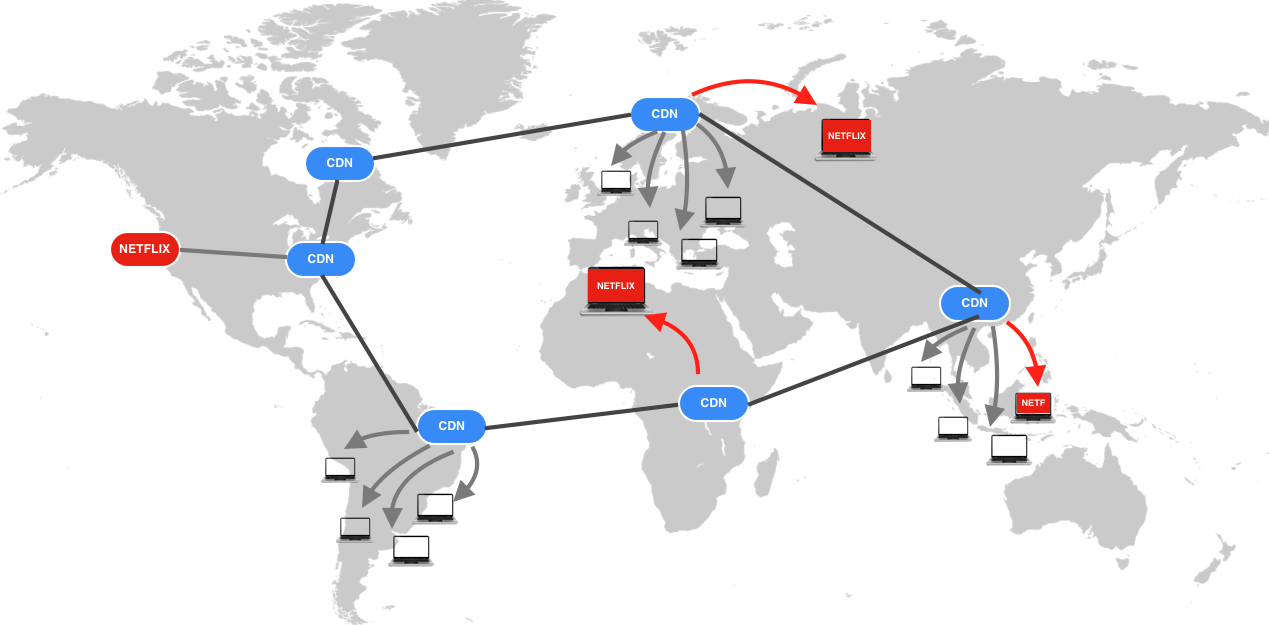
\includegraphics[scale=0.30]{map} 
%\end{center}
%\caption{\label{fig:controller}Architecture of the unified QoS metric fuzzy controller.}
%\end{figure} 
%\fi


\end{document}
